\documentclass[../main.tex]{subfiles}

\graphicspath{{../images/}}
\ifSubfilesClassLoaded{
    \twocolumn
}{}

\begin{document}

% cornell_bo_16384spp.png and dragon_1024spp.png figure
\begin{figure}[h]
    \centering
    \begin{subfigure}{0.23\textwidth}
        \centering
        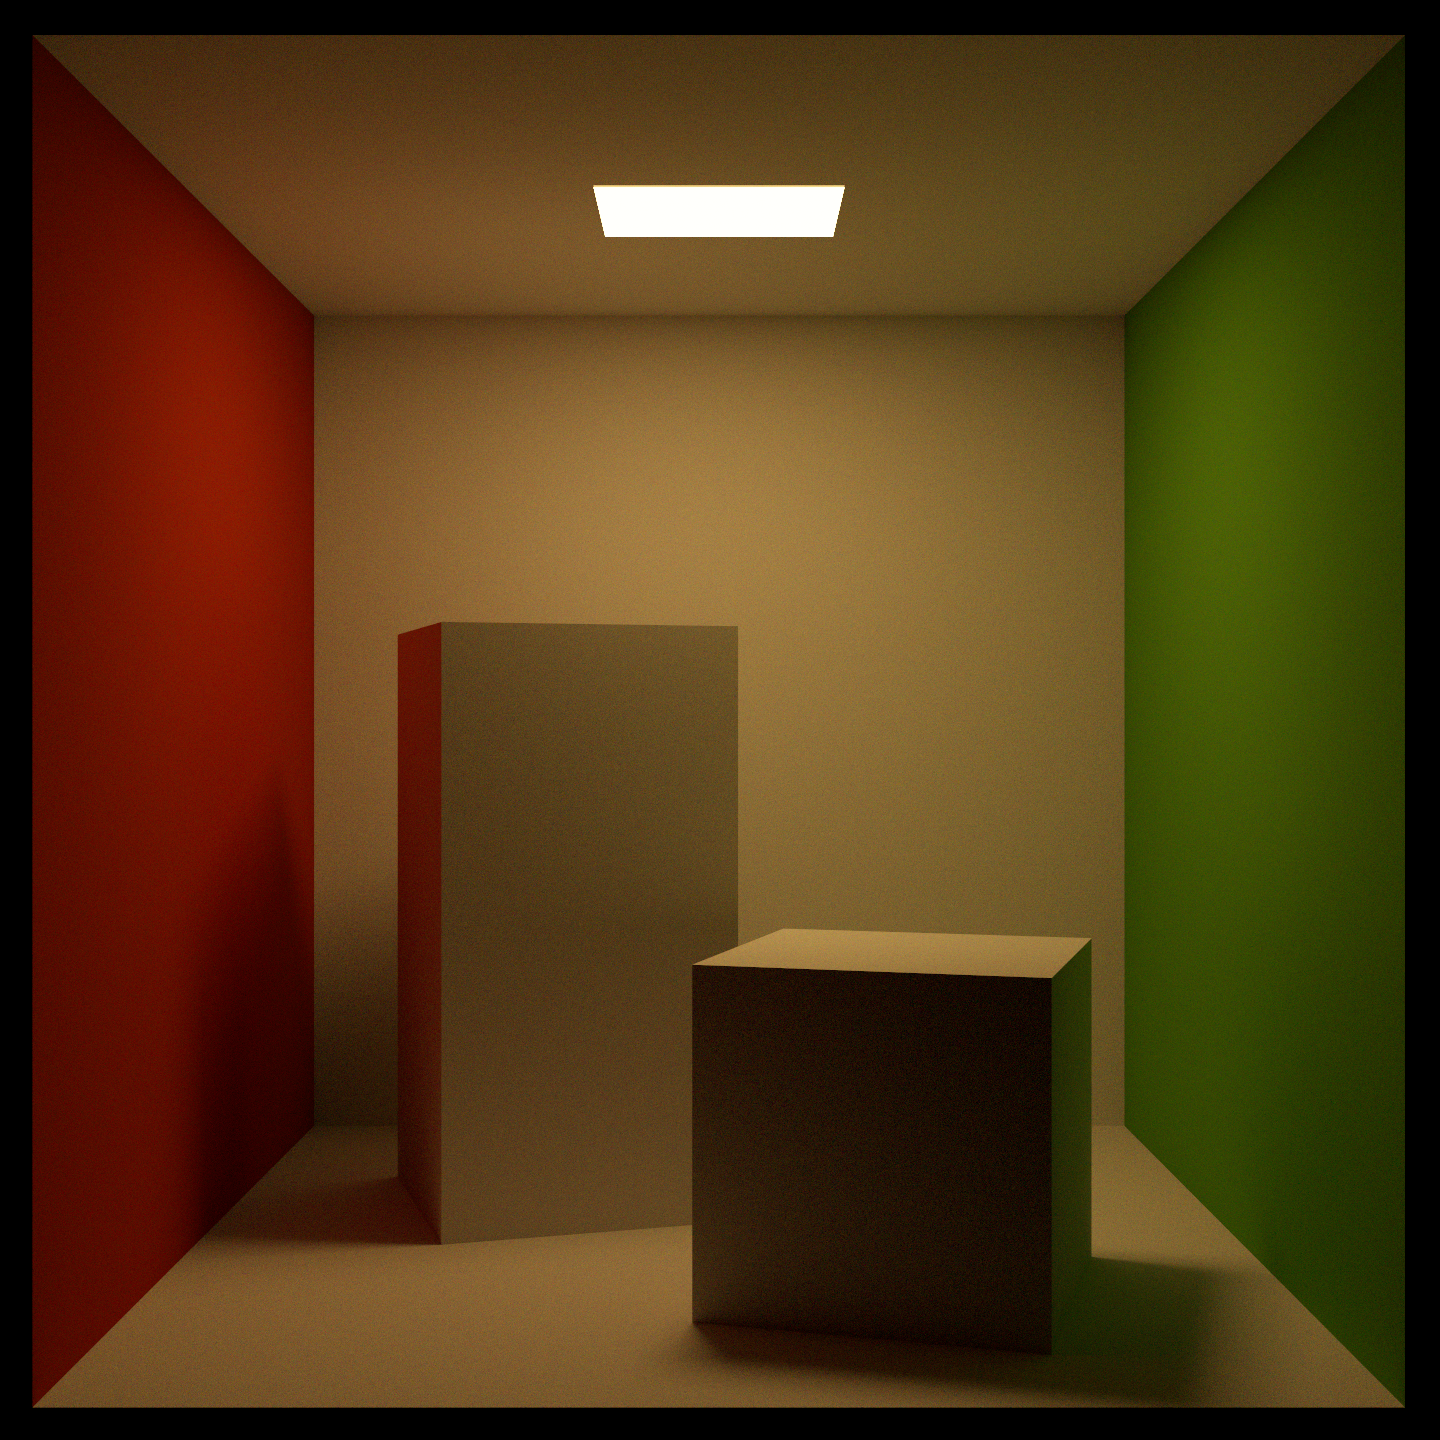
\includegraphics[width=\textwidth]{cornell_box_16384spp.png}
        \caption{Rendering time: 700s}
        \Description{Image}
        \label{fig:cornell_box_16384spp}
    \end{subfigure}
    \begin{subfigure}{0.23\textwidth}
        \centering
        \includegraphics[width=\textwidth]{dragon_1024spp.png}
        \caption{Rendering time: 15,000s}
        \Description{Image}
        \label{fig:dragon_1024spp}
    \end{subfigure}
    \caption{
        (a) Cornell box with 16,384 samples per pixel
        (b) 100,000 triangle \texttt{dragon.obj} \cite{stanford_dragon} with 1024 samples per pixel
    }
    \Description{Image}
    \label{fig:cornell_box_16384spp_and_dragon_1024spp}
\end{figure}

\section{Discussion}

Although the CRT renderer is capable of rendering a Cornell box scene with a
triangle mesh object (Figure \ref{fig:cornell_box_16384spp}), the perfomance greatly suffers for increasingly complex
triangle meshes. For simple geometry, the CRT can render the original Cornell Box
test scence with 16,384 samples per pixel in 700s compared to 12,000s for the
Donkey Kong Cornell box scene. For even more complex geometry used in professional
3D modeling software, our implementation does not scale to the same computational
speed as the PBRT GPU renderer (Figure \ref{fig:dragon_1024spp}). This is due to our CRT computing
only indirect lighting and not using any further acceleration structures to speed up the
ray-triangle intersection test. Despite the limitations of our implementation, the CRT
renderer is capable of taking \texttt{.obj} files from professional 3D modeling software
such as Blender and render physically based images using spectral data which is not readily
available as a core feature in most ray tracing software (PBRT natively supports spectral
rendering).
% \cite{IEC61966-2-1-Amd1}
% \url{https://www.iec.ch/}

% for subfile compilation
\ifSubfilesClassLoaded{%
    \nocite{*}
    \bibliographystyle{ACM-Reference-Format}%
    \bibliography{references}%
    \twocolumn
}{}
\end{document}
